\chapterimage{/11/head.jpg} % Chapter heading image
\chapter{Cosmic Microwave Background}\label{11:ch}
Attualmente, la fonte principale di informazione cosmologica è la radiazione cosmica di fondo. È un ``bagno termico di fotoni'' osservabile da qualsiasi direzione e legato al fenomeno dell'ultimo scattering dovuto alla ricombinazione dell'idrogeno ($z\approx 1100$). La scoperta da parte di Arno Penzias e Robert Wilson è stata serendipitosa, ma la radiazione era prevista teoricamente dai modelli di nucleosintesi primordiale (ai tempi si stimava $T_0\simeq 5$K). La scoperta della CMB (metà anni `60) è stata definitiva per l'abbandono del modello stazionario, che non prevede un fenomeno di creazione di tali fotoni spiegabile semplicemente. 

La CMB è il ``corpo nero più perfetto misurato in natura'', la sua temperatura è diminuita con l'espansione dell'universo ($\sim 3000 \to 2.73$ K), ma la distribuzione è rimasta quella di un corpo nero (conservazione dei fotoni). 

Oltre a questo, si è cercato di costruire strumenti sempre più sensibili per osservare piccole fluttuazioni nella distribuzione di temperatura. Inizialmente venne osservato solo il termine di dipolo dovuto al moto relativo tra noi e il sistema di riferimento comovente, rispetto al quale la CMB dovrebbe essere isotropa (rotazione terrestre, del Sole nella Galassia, moto della Galassia). Negli anni `90 il satellite COBE ha studiato le prime fluttuazioni ccon una risoluzione di $\sim 7$ gradi. 

Il problema dell'orizzonte si nota principalmente nella CMB. Si osservano regioni di cielo con temperatura quasi uniforme su scale che ai tempi non potevano essere in connessione causale. Come già discusso, il problema è stato brillantemente risolto con il modello inflazionario. 

\vspace{1em}
Osservativamente si misura la quantità: $\frac{\delta T }{T} (\theta, \phi)=\frac{T(\theta,\phi) - \overline{T}}{\overline{T}}$ e si costruiscono mappe che coprono tutto cielo. È una quantità bidimensionale e per studiare meglio le sue caratteristiche si scompone in \textit{armoniche sferiche}. Non conviene utilizzare le trasformate di Fourier come si è fatto col campo di densità perché sono legate a quantità cartesiane. Normalmente si studiano aree estese nel cielo, in caso contrario si può sempre ricorrere all'equivalente dello spettro di potenza bidimensionale. In generale si utilizza la seguente convenzione:
\begin{equation}
    \delta_T (\theta, \phi) = \sum_{l=0}^\infty \sum_{m=-l}^{l}a_{lm}Y_{lm} (\theta, \phi); \qquad Y_{lm} (\theta, \phi):= \sqrt{\frac{2l+1}{4\pi}\frac{(l-m)!}{(l+m)!}P_l^m (\cos\theta)e^{i\phi}}
\end{equation}
dove $Y_{lm}(\theta, \phi)$ è un'armonica sferica e $P_l^m$ è il polinomio di Legendre di indici $l$ e $m$ (il primo legato a un angolo sotteso, il secondo a una direzione). L'indice $l$ assume valori tra $0$ e $+\infty$ ed è legato all'inverso dell'angolo $\theta$:
\begin{itemize}
    \item $l=0$: termine di monopolo, $\theta=360^\circ $;
    \item $l=1$: termine di dipolo, $\theta=180^\circ $;
    \item $l=2$: termine di quadrupolo, $\theta=90^\circ $;
    \item $l \gg 3$: $\theta\approx 180^\circ /l$.
\end{itemize}

Analogamente allo spettro di potenza per il campo di densità: $\mathcal{P}(k)\propto \langle|\delta_k^2| \rangle $ (mediato su tutti i $k_x$, $k_y$ e $k_z$ corrispondenti a un modulo $k$), si utilizza lo \textbf{spettro di potenza angolare}: $\mathcal{C}(l) =  \langle|a_{lm}^2| \rangle$ (mediato su tutti gli $a_{lm}$ che condividono lo stesso $l$):
\begin{equation}
    \mathcal{C}(l)=\frac{1}{2l+1}\sum_{m=-l}^l a_{lm}^2
\end{equation}
che misura quanto è importante la fluttuazione di temperatura su una data scala. Come nel caso della densità, anche $\mathcal{C}(l)$ non è una vera potenza, ma una densità di potenza. Non va confuso con lo spettro energetico, che è la plankiana!

\section{Anisotropie}
Ci sono tre meccanismi principali che causano fluttuazioni di temperatura nell'universo primordiale:
\begin{enumerate}
    \item \textbf{Gravità}: un fotone che parte in una buca di potenziale perderà eneria per uscire e verrà redshiftato, il contrario avviene per i fotoni che partono dalle creste (\textit{redshift gravitazionale});
    \item \textbf{Densità}: avendo assunto fluttuazioni di tipo adiabatico, le sovradensità corrispondono a zone più calde e le sottodensità a zone più fredde: questo meccanismo agisce in modo opposto alla gravità;
    \item \textbf{Campo di velocità}: una componente di velocità lungo la linea di vista può cambiare la temperatura osservata.
\end{enumerate}
In reatà sono tutti legati al campo di densità. Le anisotropie vengono divise in due grandi categorie:
\begin{itemize}
    \item \textbf{Primarie}: originate al momento del last scattering;
    \item \textbf{Secondarie}: si creano lungo il viaggio del fotone dal last scattering fino a noi (SZ, lensing, ...)
\end{itemize}

\subsection{Termine di dipolo}
Il termine di monopolo rappresenta matematicamente la media della quantità che si sta trasformando: la media di $\delta T/T$ è $0$ per definizione. Anche il termine di dipolo, il primo osservato storicamente, non è interessante da un punto di vista cosmologico. Essenzialmente è dovuto al moto della Terra rispetto al sistema di riferimento solidale alla CMB. Gli effetti che lo caratterizzano sono principalmente due:
\begin{enumerate}
    \item Vengono catturati più fotoni nella direzione del moto: $\delta T \propto \left(1+\frac{v }{c}\cos\theta\right)$;
    \item Aberrazione relativistica dell'angolo: $\delta F \propto \delta\Omega^{-1} \propto  \left(1+\frac{v }{c}\cos\theta\right)^2$.
\end{enumerate}
Overall, si ha che l'intensità del corpo nero riscala come $\left(1+\frac{v }{c}\cos\theta\right)^3$ più un termine del secondo ordine, pertanto:
\begin{equation}
    T'(\theta)= T(\theta) \left(1+\frac{v}{c}\cos\theta \right)\left(1-\frac{v^2}{c^2}\right)
\end{equation}
Nel 1976 è stato misurata un'anisotropia di: $\delta T / T \simeq 1.3\cdot 10^{-3}$ totalmente ascrivibile agli effetti relativistici accennati. Questa corrisponde a una velocità relativa di $v\simeq 390$ km/s, includendo i noti movimenti della Terra rispetto alla Galassia e della Galassia rispetto al Gruppo Locale, si può inferire che il Gruppo Locale si muove con $v\approx 600$ km/s rispetto la CMB (si sta muovendo verso il grande attrattore, tra l'Hydra e il Centauro).

Tutto questo però prescinde dalla cosmologia e un'eventuale velocità cosmologica sarebbe trascuraile perché su scala molto grande ($180^\circ $). 

\subsection{Termini di quadrupolo e di ordini superiori}
Analogamente allo spettro di potenza, a valori piccoli/grandi di $l$ corrispondono scale grandi/piccole. Diventa fondamentale distinguere quindi le scale che si trovano dentro e fuori dall'orizzonte al momento dell'ultimo scattering (corrispondenti a $l_H$).

\subsubsection{Scale $l<l_H$ ed effetto Sachs-Wolfe}
Fuori dall'orizzonte agisce solo la gravità. Il campo di velocità è trascurabile perché la velocità è sempre sottodominante rispetto alla densità essendo più lineare. Rimangono quindi solo i primi due meccanismi:
\begin{itemize}
    \item \textbf{Gravità}: $T\propto v^2 \propto \phi \quad\rightarrow\quad \frac{\delta T }{T}\propto \frac{\delta \phi }{\phi} =\frac{\delta \phi }{c^2}$
    \item \textbf{Densità}: $\frac{\delta T }{T} \propto - \frac{\delta a}{a} = -\frac{2}{3}\frac{\delta t }{t} = -\frac{2}{3}\frac{\delta \phi }{c^2}$
\end{itemize} 
Overall, si ha la seguente relazione, nota anche come \textbf{effetto Sachs-Wolfe}:
\begin{equation}
    \frac{\delta T}{T}\propto \frac{1}{3}\frac{\delta\phi}{c^2}
\end{equation}
Questo significa che se un fotone parte da una buca di potenziale, verrà redshiftato. Regioni di sovradensità corrispondono a macchie fredde. L'inflazione prevede fluttuazioni del potenziale con un andamento piatto $\mathcal{P}(k)\propto k^{\approx 1}$, quindi ci si aspetta uno spettro angolare del tipo $\mathcal{C}(l)\propto l^{n-1}\propto l^0$ per $l<l_H$.

\subsubsection{Scale $l>l_H$ e oscillazioni acustiche}
Su scale più piccole della scala dell'orizzonte, come più volte sottolineato, la microfisica non è più trascurabile. Vi è un periodo in cui i barioni e fotoni accoppiati sguazzano nelle buche di potenziale generate dalla materia oscura già disaccoppiata. Il signor barione vorrebbe cascarci dentro, mentre la pressione di radiazione lo spinge fuori. Il massimo della gravità corrisponde alla massimo della compressione e a una velocità della particella nulla, mentre i minimi della gravità corrispondono ai massimi della rarefazione e velocità nulle (Fig. \ref{fig11:osc}a). Modellandolo come oscillatore armonico, vi è uno sfasamento di $\pi/2$ tra il massimo della gravità e il massimo della velocità. Queste due quantità avranno un andamento del tipo $\sin\theta$ e $\cos\theta$ reciprocamente. Pertanto le oscillazioni complessive in temperatura andranno come $A^2(\sin^2\theta+\cos^2\theta)=A^2$ indipendentemente dall'angolo $\theta$. Lo spettro angolare risulta quindi costante anche per $l>l_H$, ma con una diversa normalizzazione.

\vspace{1em}
Quanto detto è valido fino al momento del disaccoppiamento, qua assunto avvenire istantaneamente. I barioni, improvvisamente liberi, si trovano in diverse posizioni delle buche di potenziale che corrispondono a un $l$ e quindi $\theta$ diversi (multipli delle stesse armoniche si troveranno nella stessa posizione). In questo discorso non si è ancora considerato il contributo della gravità del barione che non più trascurabile. Questa approfondisce ulteriormente la buca di potenziale: l'oscillazione rimane sfasata di $\pi/2$, ma le due ampiezze non sono più uguali (Fig. \ref{fig11:osc}b). L'oscillazione quindi non avviene più attorno allo $0$,ma attorno a un livello dipendente dal numero di barioni. Per  lo stesso motivo si instaura una disomogeneità nei picchi. Sommati in quadratura, i picchi pari (che corripondono ai momenti di massima rarefazione) sono più bassi dei picchi dispari (che corrispondono ai momenti di massima compressione). 
\begin{definition}
    La differenza di altezza tra picchi pari e dispari è una misura diretta del numero di barioni nell'universo (Fig. \ref{fig11:cttmodelb}).
\end{definition}

\begin{figure}[H]
    \centering
    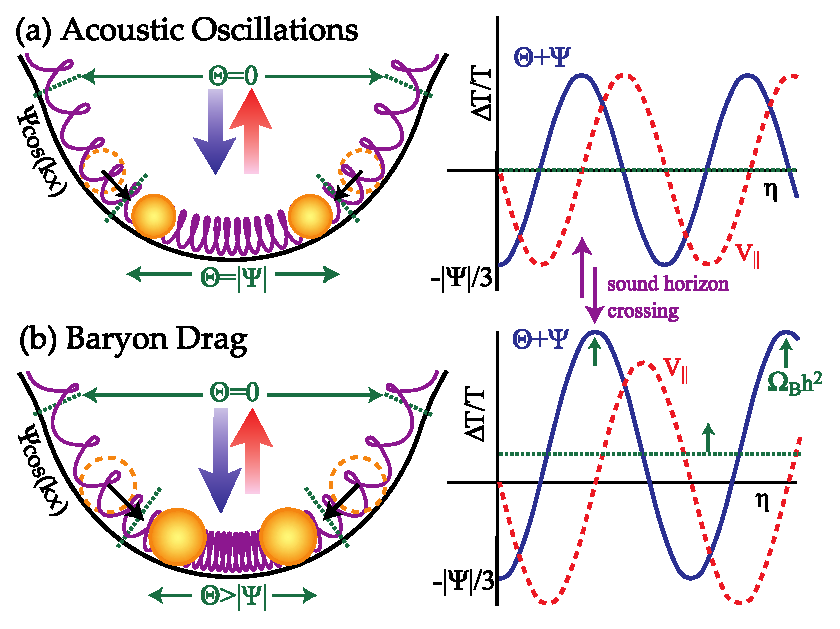
\includegraphics[width=.75 \textwidth]{Pictures/11/OscDrag.eps}
    \caption{(a) Oscillazioni acustiche tra $-\pi/2 <kx <\pi/2$. Le molle e le palline rappresentano rispettivamente pressione di radiazione e gravità. L'ampiezza delle oscillazioni vale $|\Psi|/3$ dove $\Psi$ è il potenziale newtoniano. Il blueshift dovuto alla pressione del fluido e il redshift dovuto alla gravità si bilanciano. (b)   (From: https://arxiv.org/abs/astro-ph/9604166 CITAAA)}\label{fig11:osc}
\end{figure}

\begin{figure}[H]
    \centering
    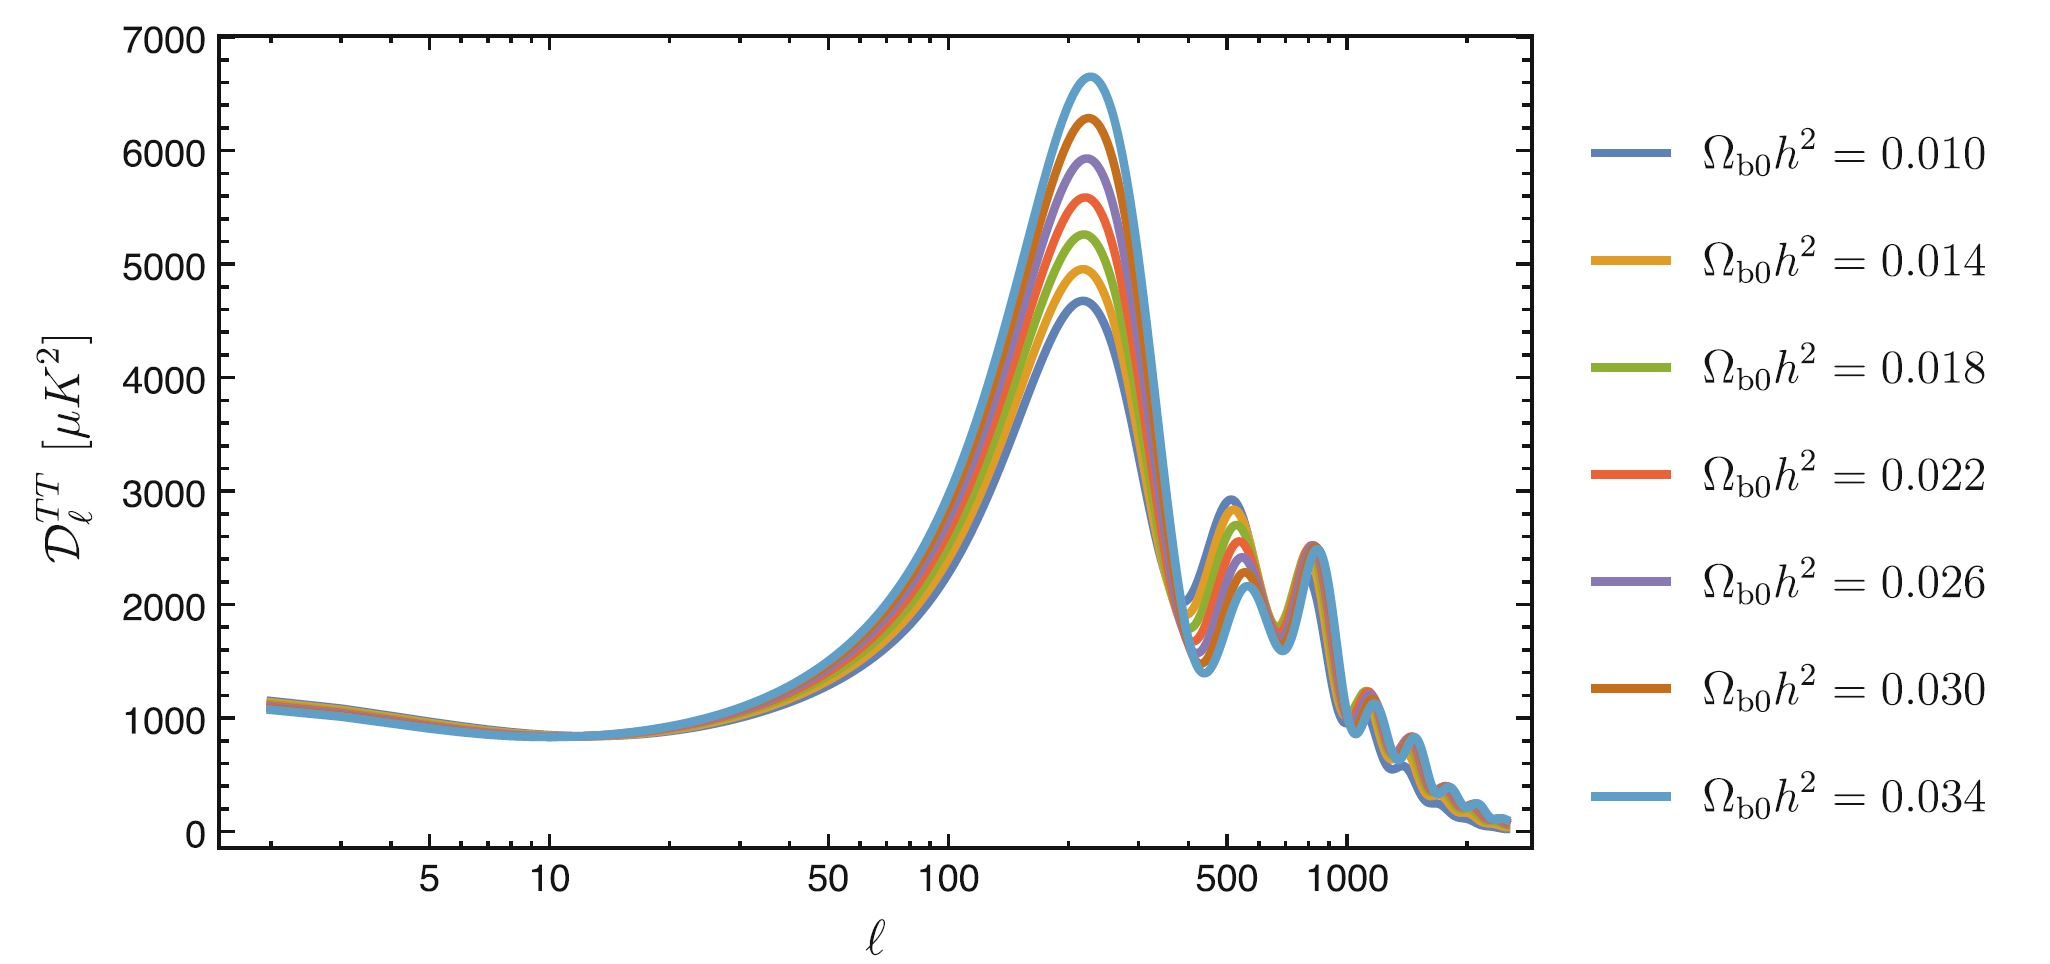
\includegraphics[width=.8 \textwidth]{Pictures/11/angspecmodel.jpg}
    \caption{Spettro angolare delle futtuazioni in temperatura modellato al variare del parametro di densità dei barioni. (FONTE Piattella CITAAAA) }\label{fig11:cttmodelb}
\end{figure}

Il primo picco è la prima scala di massima compressione dentro l'orizzonte, è quindi legata alla scala dell'orizzonte al momento dell'ultimo scattering. Le oscillazioni acustiche non possono avvenire per $l\to \infty$ perché il Sig. Silk ci ha già detto che esiste una scala di dissipazione per l'oscillazione dei barioni. Il taglio ha un andamento del tipo $l^{-4}$. Osservativamente si ha lo spettro mostrato in Figura \label{fig11:cttobs}.




\section{Anisotropie Secondarie}
Dalla superficie dell'ultimo scattering fino a noi i fotoni possono andare incontro a interazioni che modificano lo spettro angolare delle fluttuazioni primitivo. Nella \href{http://background.uchicago.edu/~whu/intermediate/intermediate.html}{pagina web del Professor Wayne Hu} è possibile trovare animazioni che rendono più chiari i concetti che verranno discussi.

\subsection{Effetto Sachs-Wolfe Integrato}
È dovuto a fluttuazioni del potenziale gravitazionale lungo la linea di vista. Viene suddiviso in tre categorie:
\begin{itemize}
    \item \textbf{Late ISW}. A livello lineare in un universo EdS la fluttuazione del potenziale gravitazionale è costante. Per universi in cui $\delta_+ \not\propto a$ (e.g, universi curvi, modelli piatti con costante cosmologica,...) si ha $\dot{\delta\phi}\neq 0$, pertanto si osservano fluttuazioni nella tempreratura dovute a questo fenomeno;
    \item \textbf{Early ISW}. L'equivalenza avviene a $z_{eq}\approx 6000$, la ricombinazione a $z_{rec}\approx 1500$. Anche se piccolo, vi è un intervallo temporale in cui una bassa, ma non nulla densità di radiazione determina un andamento: $\delta_+ \propto \gtrsim a$ generando un $\dot{\delta\phi}> 0$. Questi primi due effetti devono avvenire entro l'orizzonte al momento in cui si verificano. L'early rompe le scatole su scale leggermente a sinistra del primo picco, il late a $z\approx 1\div 2$, ossia a scale grandi ($l$ bassi) (Fig. \ref{fig11:secanisot}).
    \item \textbf{Rees-Sciama}. È dovuto alla non linearità. Se, nel tempo, la buca di potenziale / vuoto si approfondisce / livella più del dovuto il fotone subisce una predita / guadagno netto di energia. 
\end{itemize}
Questi effetti sono dovuti alla distribuzione della materia, per amplificare il segnale cosmoogico vengono osservati cross-correlando la CMB e la struttura su larga scala. 

\begin{figure}[H]
    \centering
    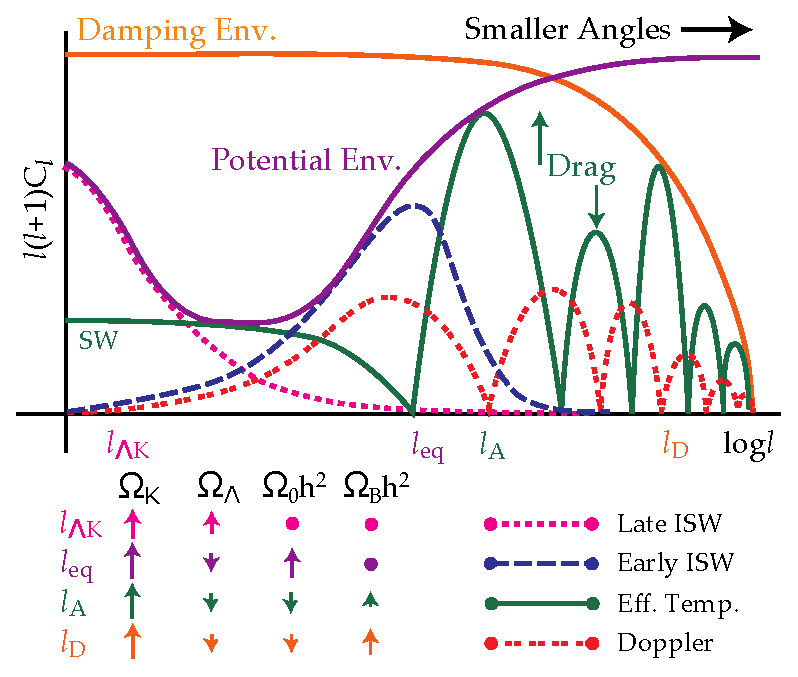
\includegraphics[width=0.75 \textwidth]{Pictures/11/secanisotropies.eps}
    \caption{Spettro delle anisotropie su scala logatitmica. L'andamento di $l_{\Lambda K}$ e di $l_{eq}$ genera il pateau di Sachs-Wolfe (SW). Il baryon drag intensifica i picchi dispari e può essere una probe per le fluttuazioni all'ultimo scattering e/o $\Omega_b h^2$.} \label{fig11:secanisot}
\end{figure}

\subsection{Lensing gravitazionale}
Anche questo dipende dalla distribuzione della materia. Non cambia le temperature dei fotoni, ma soltanto il tragitto dei fotoni. Pertanto, il lensing sfoca le mappe di temperatura. 

\subsection{Effetto Sunyaev-Zeldovich}
Il fotone può anche interagire con la materia reionizzata dai fenomeni di galaxy evolution a partire da $z\approx 5$. Essendo di bassa energia interagisce con gli elettroni caldi per effetto compton inverso. Questo fenomeno può avvenire globalmente su grandi scale e localmente negli ammassi di galassie, lobi delle radio galassie e così via\dots Naturalmente questo fenomeno può avvenire solo su scale non più grandi dell'orizzonte, generalmente $l>10$. Con il passare del tempo la densità barionica media e quella della radiazione decrescono, quindi la probabilità di avere scattering inverso sarà sempre minore. Ulteriori dettagli sono riportati in Figura \ref{fig11:sz}.



\section{Risultati osservativi}
Come già discusso, \textbf{la posizione (non il valore) del primo picco} è legata alla scala dell'orizzonte al momento dell'ultimo scattering. Il valore: $R_H(z_{LS})=a(z_{LS})\int_0^{t_{LS}}c \; \d{t} / a(t)$ può esssere in buona approssimazione calcolato per un universo EdS. Questa quantità può essere utilizzata come un righello standard. L'angolo sotteso da questo righello dipende dalla geometria (Fig. CITAAAA): $\Omega_k = 1-\Omega_{TOT}$. All'aumentare di $\Omega_k$ (universo aperto) la scala diventa più piccola e l'intero spettro shifta rigidamente verso $l$ grandi. La posizione osservata (per la prima volta con l'esperimento BOOMERanG) del primo picco, $l=220$, corrisponde esattamente a una geometria piatta.

\begin{definition}
    L'evidenza più importante della piattezza dell'universo è aver osservato un angolo sotteso dal raggio dell'orizzonte al momento dell'ultimo scattering corrispondente a $l=220$ ($\theta \approx 1^\circ$), esattamente come previsto da una geometria piatta ($\Omega_{TOT}=1$). Con lo spettro di potenza della materia si osservava invece una combinazione di $\Omega_m$ e $H$ perché il momento dell'equivalenza è altamente determinato dalla quantità della materia.
\end{definition}

La \textbf{differenza di altezza tra i picchi dispari e i picchi pari} si acuisce all'aumentare di $\Omega_b$. Questa misura viene fatta per ogni coppia di picchi adiacenti, ma per effetto della diffusione si ha più segnale tra il primo e il secondo. Il fit dei dati di Plank ha restituito: $\Omega_b h^2 = 0.022$, che corrisponde a $\Omega_b =0.045$ assumendo $H_0=70$ km/s/Mpc, oppure $\Omega_b =0.049$ assumendo $H_0=67.4$ km/s/Mpc (come derivato dai dati di Plank). Entrambi consistenti col valore derivato dalla nucleosintesi. La dipendenza dalla costante di Hubble deriva dalla definizione di $\rho_{crit}$.

A \textbf{$l$ piccoli} si può misurare il livello di normalizzazione dello spettro di pontenza (nemmeno l'inflazione riesce a predirlo!), l'indice spettrale delle perturbazioni primordiali $n_s$ e l'effetto Sachs-Wolfe integrato dovuto a un'eventuale curvatura dell'universo e/o alla presenza di energia oscura (la quale sposta anche debolmente il primo picco verso sinistra). Per osservare \textbf{$l$ grandi}, quindi il regime di dissipazione, è necessario avere un'ottima sensibilità degli strumenti. Attenzione, $\mathcal{C}(l)$ si ottiene mediando su tutti gli $m$ possibili: è semplice osservare $l$ piccoli, ma si ha bassa statistica (grandi errori); è più complesso osservare $l$ grandi, ma si ha molta più statistica.

Può verificarsi anche una \textbf{soppressione della potenza ad alti multipoli}. Questo è dovuto principalmente alla profondità ottica e al redshift della reionizzazione e in secondo luogo alle onde gravitazionali. Questi fenomeni sono visibili anche studiando la polarizzazione della CMB. 

Le prime osservazioni delle fluttazioni cosmologiche, predette e richieste dai modelli di formazione delle strutture, $\delta T / T \simeq 10^{-5}$ sono state osservate da COBE nel 1992. In seguito, fu lanciato dall'Antartide l'esperimento BOOMERanG, sfruttando l'effetto dei venti per rimanere in volo diversi giorni su un'orbita più o meno circolare. Non venne fatta una mappa all sky, ma su una regione piccola di $25^\circ $ con una risoluzione e sensibilità tale da osservare la posizione del primo picco. Per la prima volta venne osservato $\Omega_0 =1$. WMAP (americano) e Plank (europeo) vennero progettati a partire dal 1992, il primo fu lanciato nel 2003, il secondo nel 2009. In realtà, alle frequenze di osservazione, non si vede nulla di cosmologico. I contributi di \textit{foreground} dovuti al sincrotrone e alla polvere termale (cit.) sono sottodominanti soltanto tra 30 e 100 GHz (Fig. \ref{fig11:cmbsporca}). Una volta mappata bene la loro distribuzione energetica è possibile modellarli e sottrarli per isolare il segnale cosmologico.

\begin{figure}[H]
    \centering
    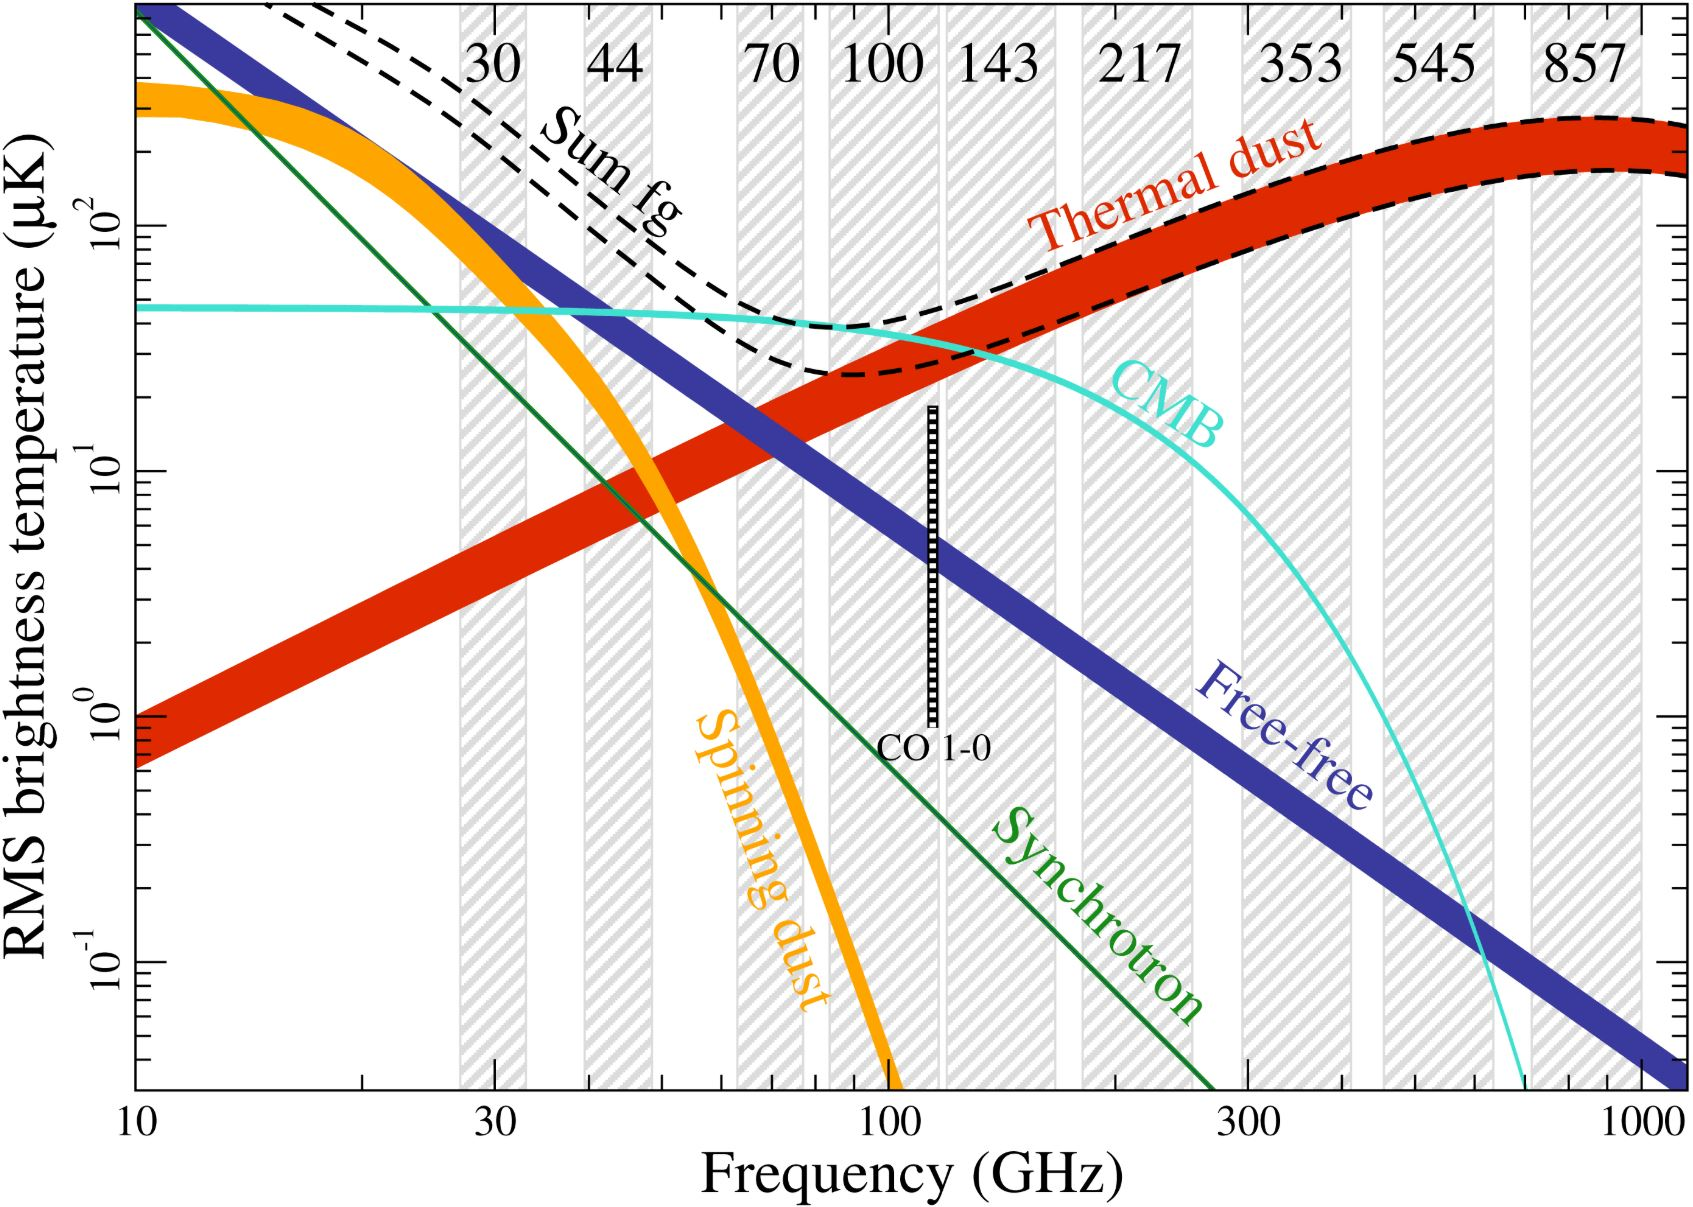
\includegraphics[width=0.65 \textwidth]{Pictures/11/falsecmb.jpg}
    \caption{Spettro angolare delle futtuazioni in temperatura teorico (linea continua) e multipoli osservati tramite la CMB (punti). Le bande shaded sono quelle utilizzate da Planck per mappare, modellare e sottrarre le componenti fastidiose per i cosmologi, ma importanti per i radioastronomi (From: ESA).}\label{fig11:cmbsporca}
\end{figure}

A questo punto la CMB si scompone in multipoli, mediando su tutti gli $m$ possibili su ogni scala corrispondente a $l$. L'ultima misura del team di Plank è riportata in Figura \ref{fig11:cttobs}. 


\begin{figure}[H]
    \centering
    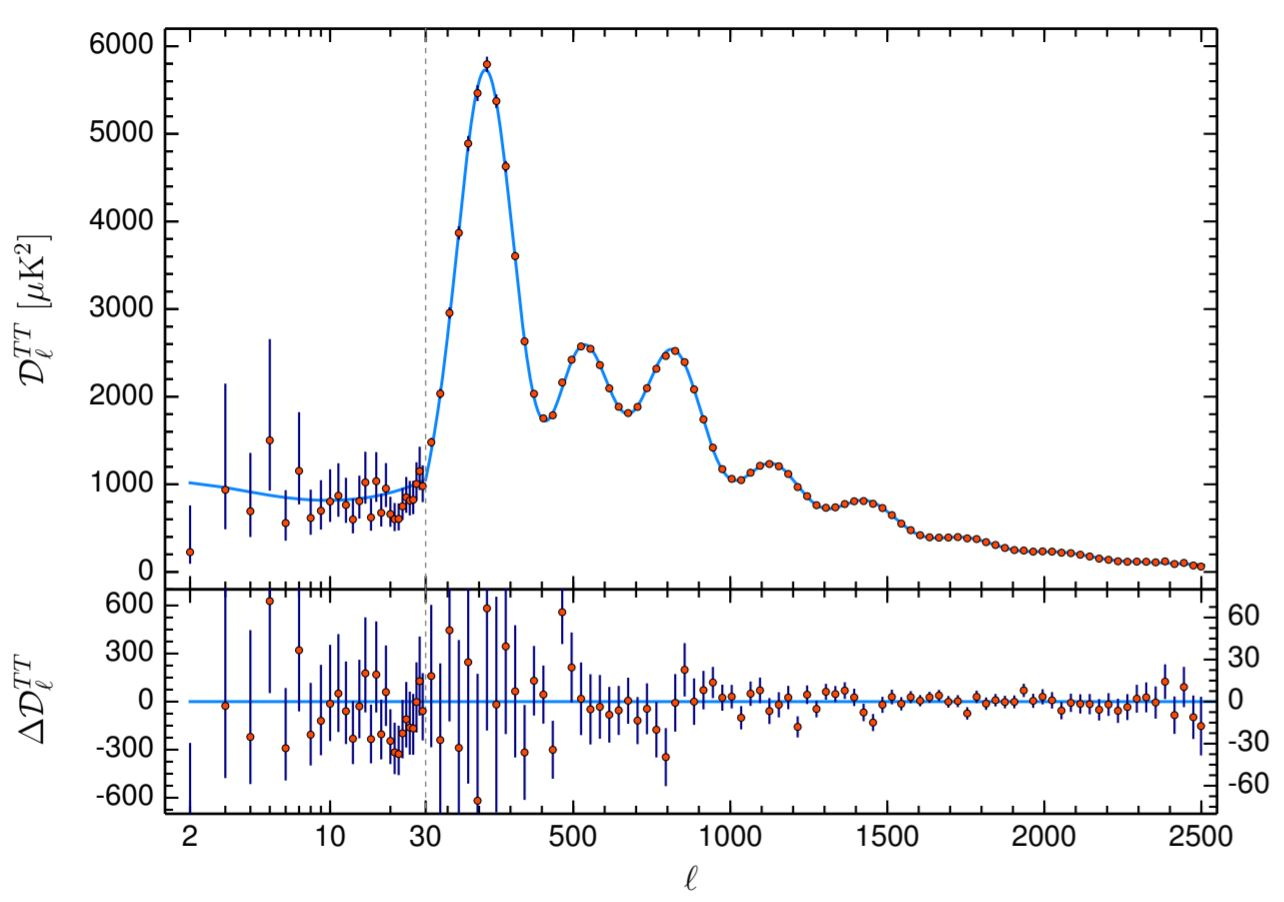
\includegraphics[width=0.72 \textwidth]{Pictures/11/angspecobs.jpg}
    \caption{Spettro angolare delle futtuazioni in temperatura teorico (linea continua) e multipoli osservati tramite la CMB (punti). Qui, $\mathcal{D}^{TT}_l:= l(l+1)\mathcal{C}_l / (2\pi)$ (From: Plank 2018 CITAAAA).  }\label{fig11:cttobs} 
\end{figure}
Chi ha l'occhio molto attento può notare qualche problemino qua e là con il modello ($l=5$, $l\approx 20$, attorno al primo picco, ...). Si parla di \textit{anomalie}. Si è arrivati più o meno ad osservare il settimo picco, $l\simeq 2500 \leftrightarrow \theta \simeq 0.07^\circ$. Notare che la scala è logaritmica per $l<30$ e lineare per $l>30$. Il fit dei dati restituisce constraints sui sei principali parametri cosmologici (numero minimo dei prarametri possibile) e quattro parametri importanti derivati:
\begin{figure}[H]
    \centering
    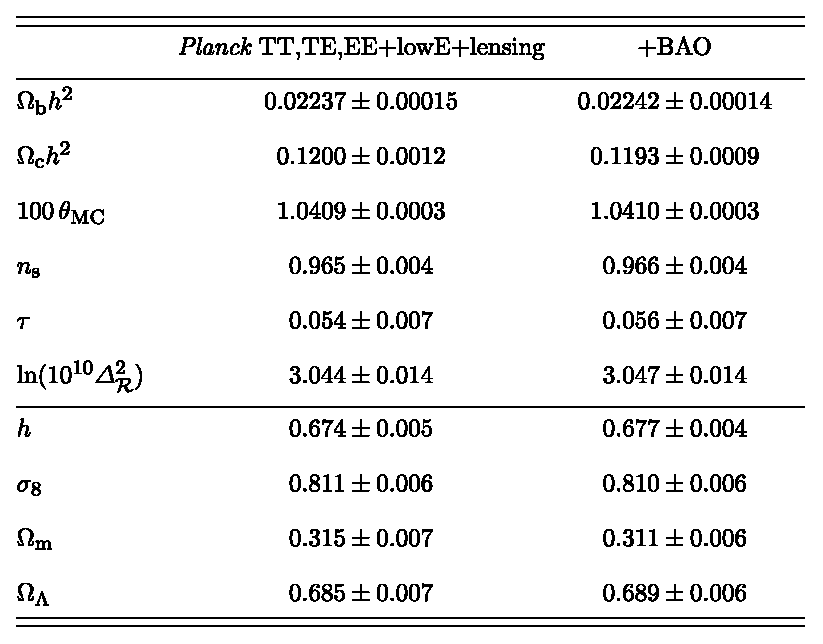
\includegraphics[width=0.65 \textwidth]{Pictures/11/planktable.eps}
\end{figure}
I sei parametri del fit sono rispettivamente: $\Omega_b h^2$, $\Omega_{DM} h^2$, 100$\times$ la scala dell'orizzonte sonoro al disaccoppiamento, indice spettrale delle perturbazioni primordiali, profondità ottica dovuta alla reionizzazione (è un segnale di disturbo) e normalizzazione dello spettro primordiale. Tra i parametri derivati vi sono: $H_0$, $\sigma_8$, $\Omega_m$ e $\Omega_\Lambda$. Inoltre con altri dati esterni, si può inferire una stima della somma delle masse dei diversi tipi di neutrini: $\sum m_\nu <0.13$ eV (ancora consistente con zero). Si può anche testare una delle ipotesi dell'inflazione: la gaussianità delle perturbazioni ($f_{NL}=0$). Si osserva una leggera e trascurabile deviazione dalla gaussianità a $z\sim 1000$, con un valore di $f_{NL}\in(-60,+60)$. Questa misura, assieme alla quantità $\d{n_s}/\d{\ln k}\in (-0.03, 0.015)$ ha comunque permesso di scartare moltissimi modelli. Infine si può studiare se le perturbazioni sono adiabatiche come è stato fino ad ora assunto (porebbero essere isoterme, di isocurvatura, ...): la deviazione di quantifica tramite la quantità $\alpha$. Planck ci assicura che $\alpha \simeq 0$ (al massimo un po' di isocurvatura). 

Una volta caratterizzati completamente gli effetti cosmologici si possono estrarre informazioni sull'effetto Sachs-Wolfe integrato correlando la CMB e la struttura a larga scala. Come ci si aspetta dal modello $\Lambda$CDM, il potenziale gravitazionale varia a redshift bassi (dark energy). Lo stesso vale per l'effetto di lensing subìto dai fotoni della CMB. 

Ad oggi ci sono due parametri che danno problemi: $H_0$ come già discusso e $\sigma_8$ (problema interno ai dati di Planck); sugli altri c'è buona convergenza con altri osservabili astrofisici. In particolare il valore di $\sigma_8$ misurato direttamente tramite la CMB è in contrasto con il valore di $\sigma_8$ che si ricava utilizzando campioni di ammassi estratti dalla CMB stessa grazie all'effetto SZ. La differenza può essere lenita dalla presenza dei neutrini.

\begin{figure}[H]
    \subfloat[]{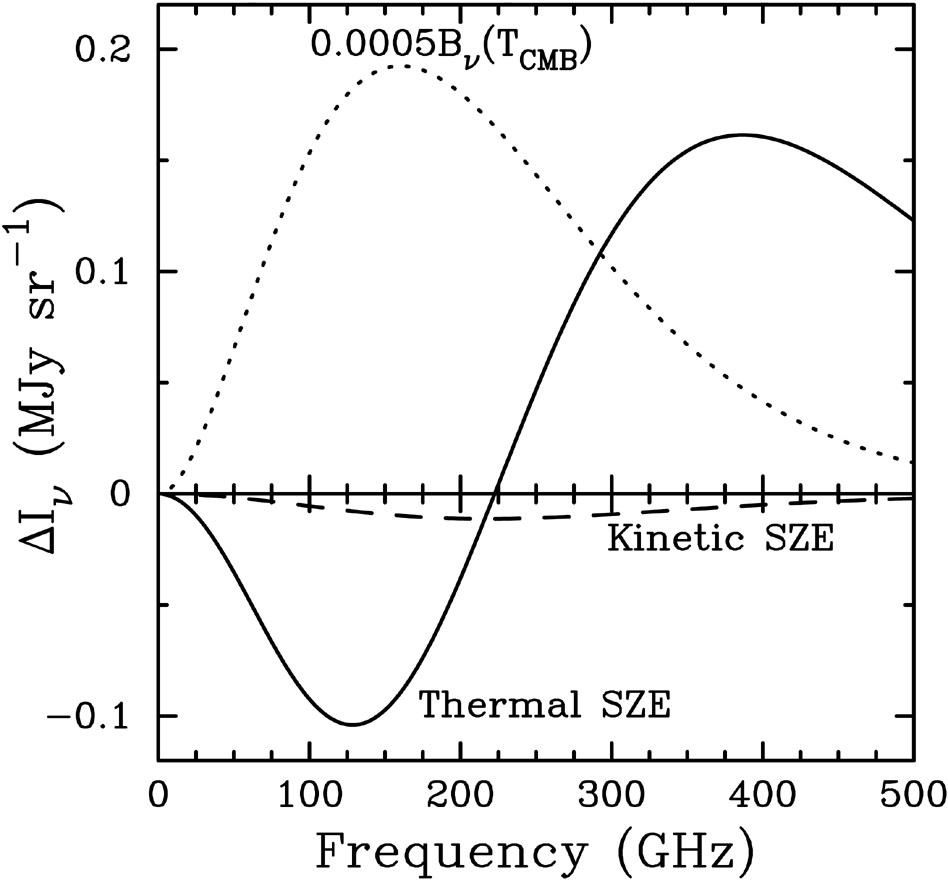
\includegraphics[width=.415\textwidth]{Pictures/11/sz.jpg}}$\;\;$
    \subfloat[]{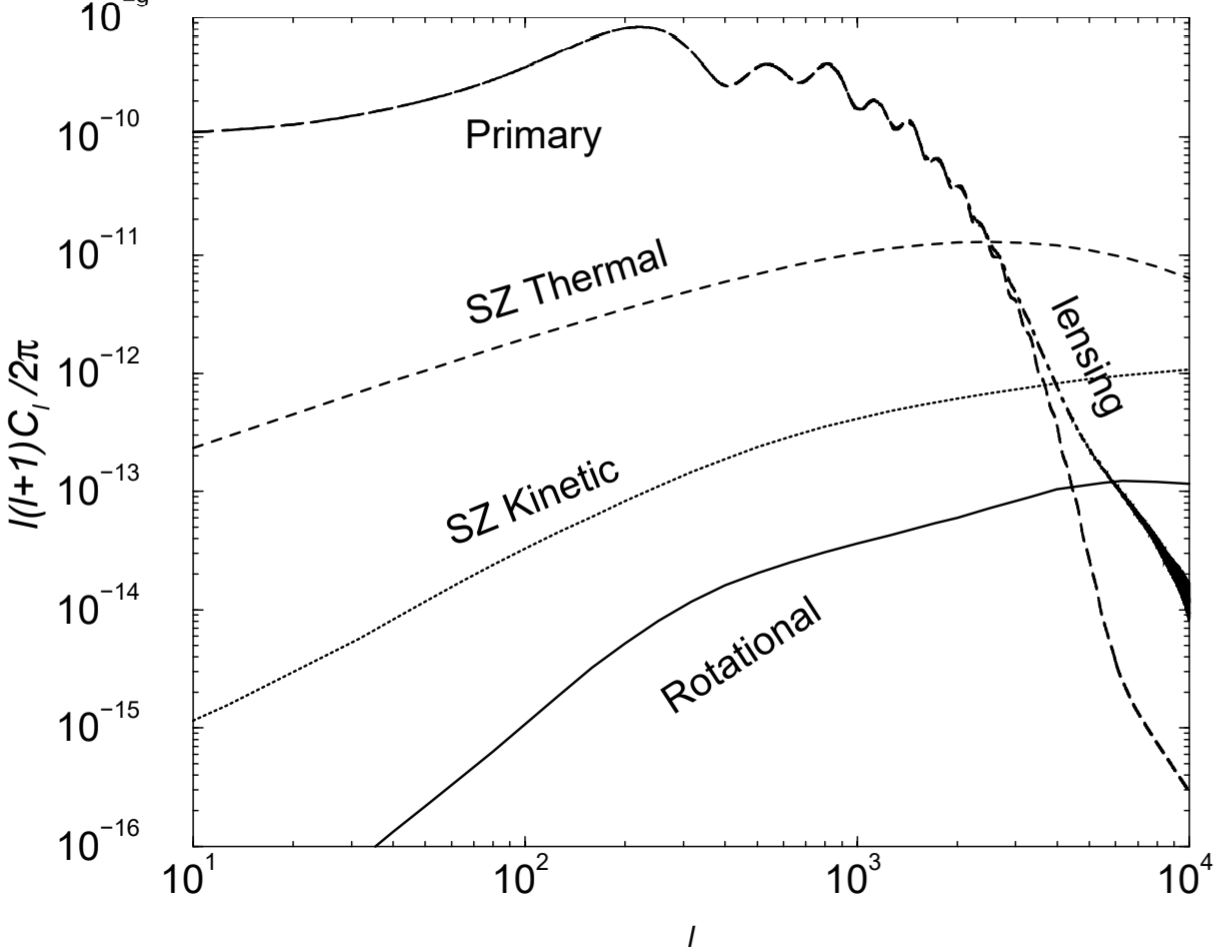
\includegraphics[width=.5\textwidth]{Pictures/11/szang.jpg}}
    \caption{(a) Risultato netto dell'effetto SZ sulla CMB. Il corpo nero della CMB è upscatterato a energie maggiori. Osservando la deformazione del corpo nero $\Delta I_\nu$ si nota che il turnover è a $\nu_t \simeq 217$ GHz.  (From: J. Carlstrom); (b) L'effetto SZ agisce su $l$ grandi ed è dovuto a tre fenomeni, di cui quello termico è il più importante (From: Kinetic Sunyaev-Zeldovich Effect from Halo Rotation)} \label{fig11:sz} 
\end{figure}


\subsection{Polarizzazione}
L'osservazione dello \textbf{spettro angolare del segnale di polarizzazione} è stata la vera rivoluzione del satellite Planck rispetto ai suoi predecessori. Ci si aspetta una polarizzazione della radiazione a causa delle proprietà dello scattering Thomson: l'onda scatterata è polarizzata perpendicolarmente al piano di incidenza. La CMB è polarizzata al 10\% a causa dello scattering degli elettroni liberi sulla superficie dell'ultimo scattering (fisicamente, si ha un segnale non nullo sulla scala di $90^\circ$ che corrisponde ad avere polarizzazione lineare). Lo spettro di polarizzazione è in fase con il campo di velocità, quindi è in antifase con lo spettro angolare e ha un valore di normalizzazione pari al 10\%. La reionizzazione introduce effetti di polarizzazione locale, che non hanno nulla di cosmologico. 

Le osservazioni di Plank hanno comfermato il modello dell'oscillatore armonico e hanno sfruttato queste informazioni per porre migliori constraints sui parametri cosmologici. La polarizzazione può essere scomposta tramite gli equivalenti dei parametri di Stokes che tengono conto della direzione di propagazione dell'onda: i modi $E$ e $B$. I primi hanno rotore nullo (traslazioni), i secondi tracciano le rotazioni. Si possono avere diversi tipi di fluttuazioni. Le fluttuazioni di densità sono scalari e generano soltanto modi $E$, quelle del campo di velocità (trascurabili, decadono  velocemente) sono di tipo vettoriale. Le onde gravitazionali sono fluttuazioni di tipo tensoriale e generano anche modi $B$. Misurando quindi i modi $B$ si possono misurare le onde gravitazionali primordiali. 

La polarizzazione $E$ è stata ben misurata, anche sfruttando la cross-correlazione tra il segnale in temperatura e il modo $E$, $TE$. A oggi, 3 gennaio 2020, non c'è alcuna evidenza di onde gravitazionali primordiali. 


\begin{figure}[H]
    \centering
    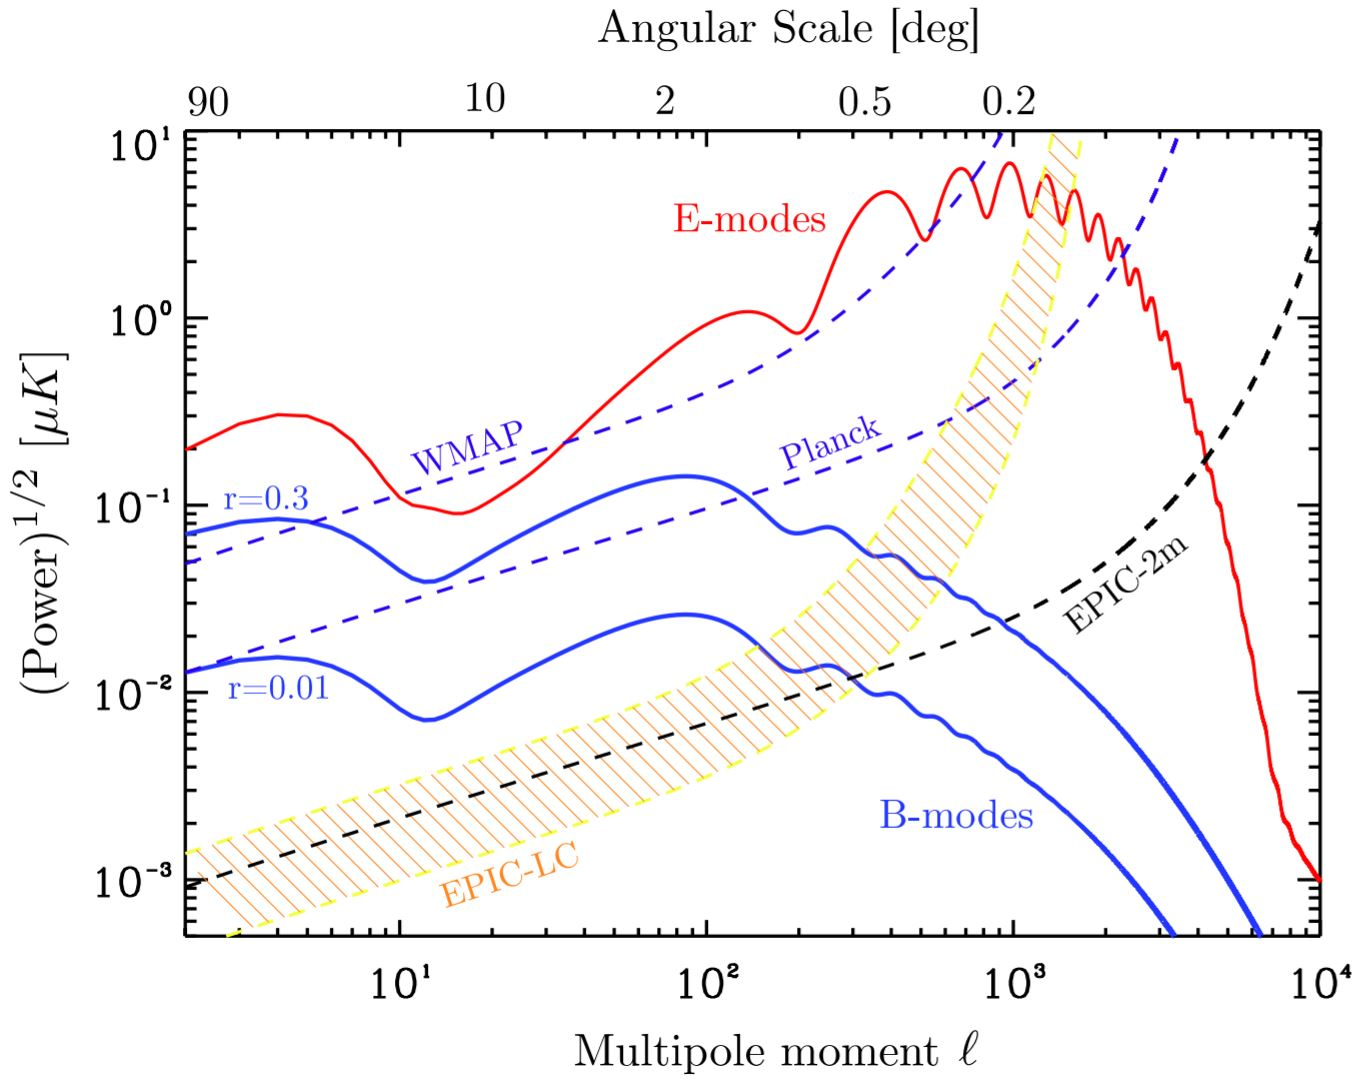
\includegraphics[width=0.7\textwidth]{Pictures/11/eb.jpg}
    \caption{Spettro di potenza per i modi $E$ e $B$. Il valore $r$ è il \textit{tensor-to-scalar ratio}. Sono mostrati i livelli di sensitivity di WMAP, Plank e quella prevista per CMBPol (EPIC-LC e EPIC-2m), non costruito (from: https://arxiv.org/abs/0811.3911).}
\end{figure}




\subsection{Oscillazioni acustiche barioniche (BAO)}
Sono una delle prove fondamentali che svolgerà Euclid. I picchi sullo spettro angolare della CMB (dovuti alle oscillazione acustiche dei barioni nelle buche di potenziale della materia oscura) lasciano un'impronta sulla distribuzione a grande scala. Osservandole, si può misurare come varia il righello standard dell'orizzonte cosmologico al variare del redshift. 

A $z$ molto alti non interessa la cosmologia, ma solo la geometria. A $z$ diversi si può tracciare l'espansione dell'universo ricavando $H(z)$, utilizzando la distanza di diametro angolare e non quella di luminosità. L'\textbf{orizzonte sonoro} (i fotoni, avendo sul groppone i fotoni hanno $v<c$) al momento dell'ultimo scattering è stato misurato da Plank e vale $s=(4.53\pm 0.06)\cdot 10^{24}$ m, ossia $\sim 150$ Mpc.
Ci si aspetta che in corrispondenza dei picchi della CMB ci siano anche piccole oscillazioni nello spettro della materia (Fig. \ref{fig11:bao}), dell'ordine del 5\%. 

Il fenomeno può essere semplificato come segue. Si consideri una singola perturbazione nell'universo primordiale: la pressione di radiazione spinge i barioni e i fotoni verso l'esterno della buca di potenziale formando una shell, l'espansione continua per $\sim 10^5$ yr. A questo punto la temperatura dell'universo è scesa a tal punto da consentire la ricombinazione dell'idrogeno. La radiazione, ora disaccoppiata, fluisce via e si omogenizza. La distribuzione di materia barionica ha quindi perso il supporto che le garantiva l'espansione e rimane in stallo su una shell di raggio $\sim 100$ Mpc. Allo stesso tempo la buca di potenziale della dark matter comincia a richiamare verso il centro della perturbazione la materia barionica. L'evoluzione dell'universo determina una crescita delle perturbazioni fattore $\sim 1000$, ma nella configurazione di equilibrio della materia dark e barionica rimane una feature legata alla dimensione della shell della materia barionica. 

La prima evidenza osservativa di BAO è ad opera di Eisenstein e collaboratori (Fig. \ref{fig11:baoobs}), che analizzando la funzione di correlazione delle galassie della SDSS hanno trovato la feature a circa $100 h^{-1}$ Mpc.

\begin{figure}[H]
    \centering
    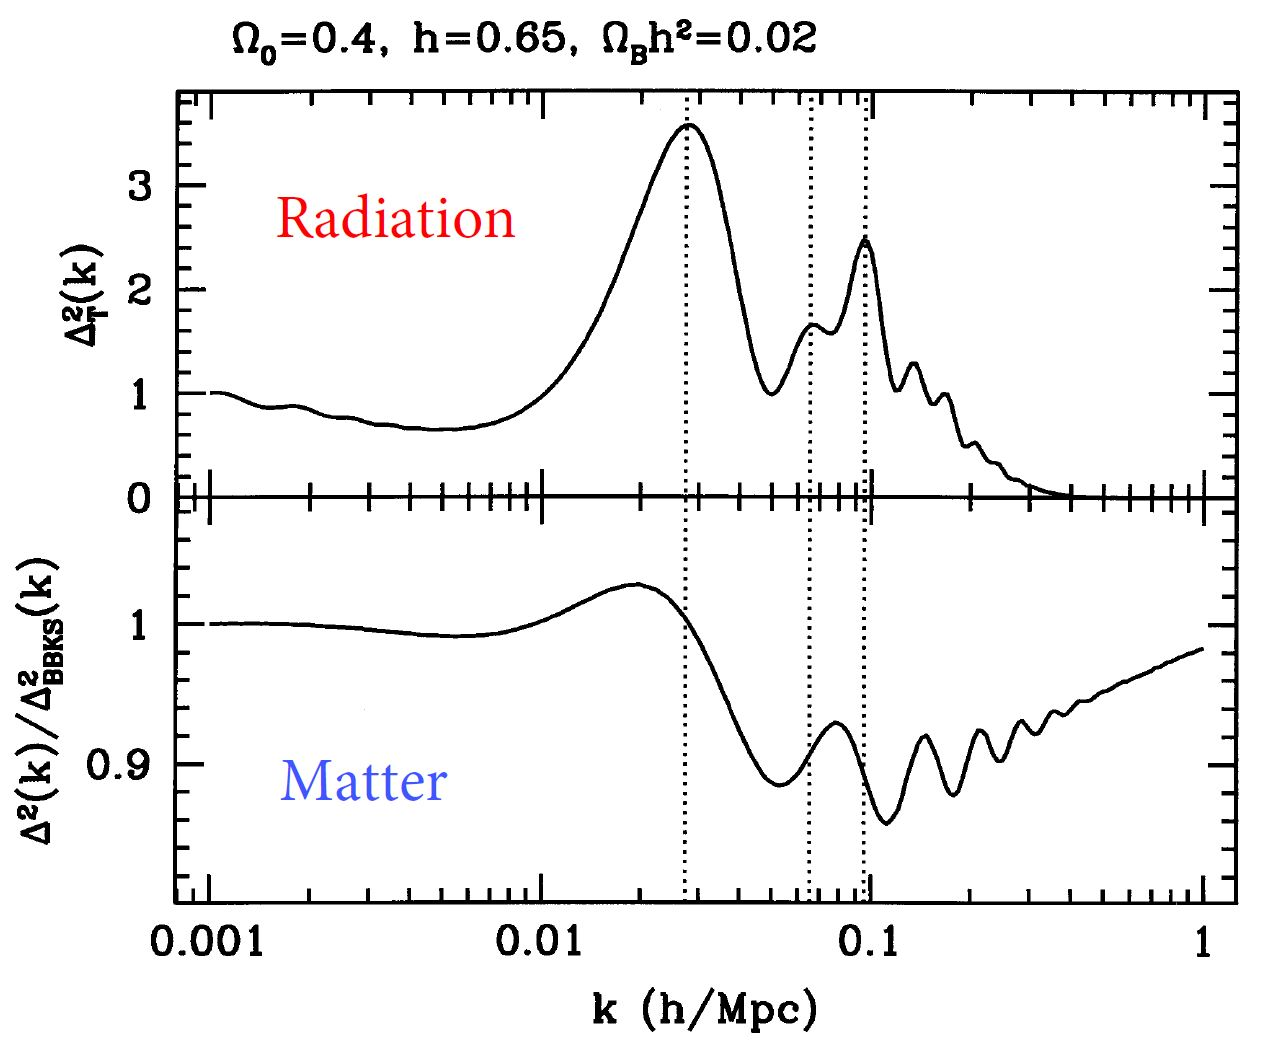
\includegraphics[width=0.7\textwidth]{Pictures/11/BAO.jpg}
    \caption{Spettro di potenza per CMB (radiazione) e LSS (materia). Non assomigliano a quelli visti perché hanno diverse normalizzazioni. (from: Baryonic signatures in large-scale structure).}\label{fig11:bao}
\end{figure}

\begin{figure}[H]
    \centering
    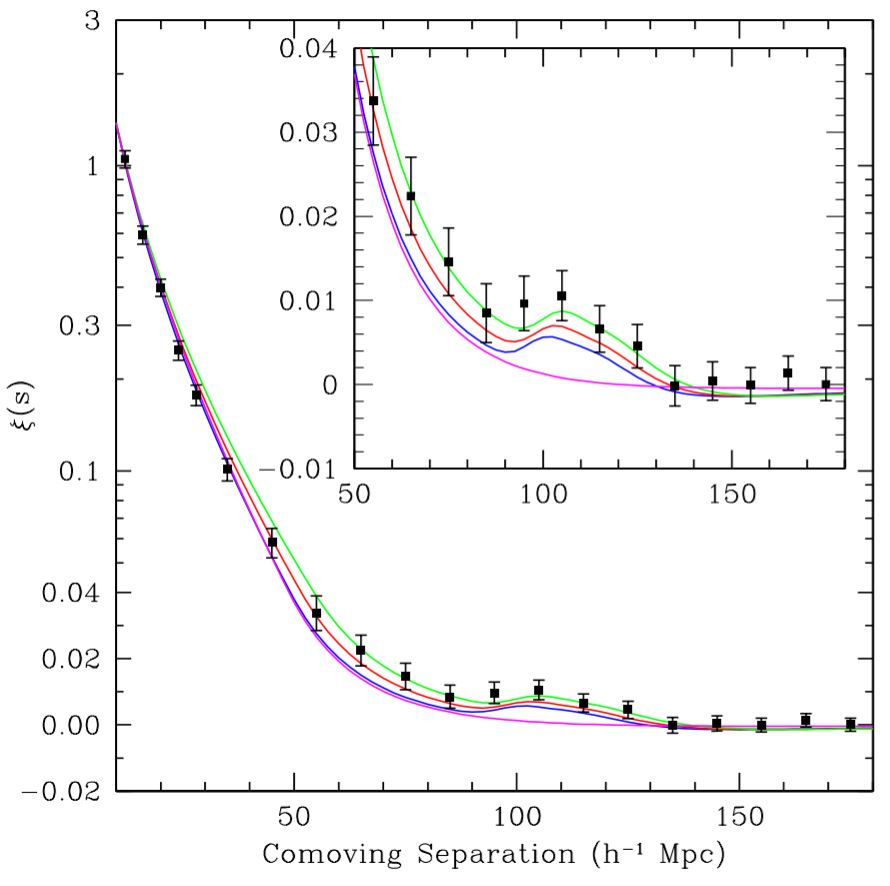
\includegraphics[width=0.7\textwidth]{Pictures/11/baoobs.jpg}
    \caption{Funzione di correlazione nello spazio dei redshift costruita dal campione SDSS LRG. Il bump è statisticamente significativo. (from: DETECTION OF THE BARYON ACOUSTIC PEAK IN THE LARGE-SCALE
    CORRELATION FUNCTION OF SDSS LUMINOUS RED GALAXIES
    ).}\label{fig11:baoobs}
\end{figure}

\textit{Complimenti per essere arrivati fino a qui, grazie per l'attenzione e speriamo che Euclid non cambi troppo le carte in tavola. A seguire qualche spunto per approfondire i temi trattati}.

\vspace{1em}
\begin{flushright}
LBL, 2020
\end{flushright}